\chapter{Introduction}

This chapter mainly provides a brief introduction to the entire project. Section \ref{bckgrd} gives the background of the project and some basic concepts. Section \ref{prodef} defines the problems of this project to be solved. Section \ref{fcswrk} gives a brief introduction to the proposed new model. Section \ref{thsorg} gives the structure of this thesis for the convenience of readers.

\section{Background}\label{bckgrd}

In this section, the background of this project is introduced. Subsection \ref{arlimg}, \ref{imgseg} and \ref{geosha} focus on aerial images, image segmentation and the segmentation with geometry respectively.

\subsection{Aerial Image}\label{arlimg}

An aerial image is a projected image which is ``floating in air'', and cannot be viewed normally. It can only be seen from one position in space, often focused by another lens (from Wikipedia). In this project, aerial images generally refer to satellite images, which are taken from satellites flying around the earth. These kind of images have an extremely wide range of applications in the field of geographical surveying and mapping. It can not only clearly depict the terrain but can also show the structure and the layout of the city. Furthermore, it can also provide services such as land use status and remote sensing monitoring.

Nowadays, many buildings are constantly being updated in real life and many landscapes are changing with natural activities. Therefore, electronic maps need to be updated accordingly, and aerial images can provide those maps with important references. Figure \ref{fig:egsatimg} shows two examples of aerial images.

\begin{figure}[!h]
	\centering
	\subbottom[an area of Zurich\label{fig:egzurich}]{
		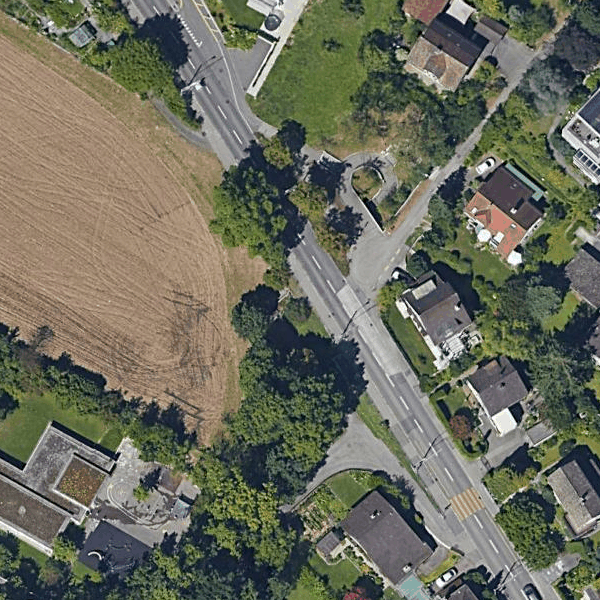
\includegraphics[width=\figfig\textwidth]{1-00-0.png}
	}
	\subbottom[an area of Chicago\label{fig:egchicago}]{
		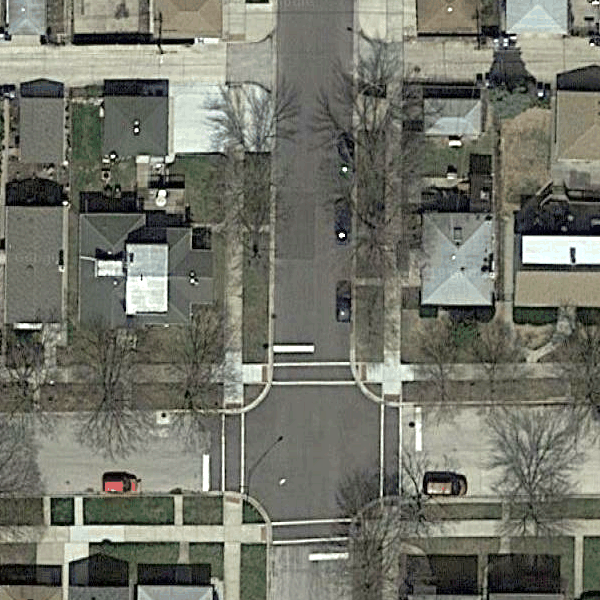
\includegraphics[width=\figfig\textwidth]{1-00-1.png}
	}
    \caption[Example of two satellite images]{Example of two satellite images.}
	\label{fig:egsatimg}
\end{figure}

\subsection{Image Segmentation}\label{imgseg}

In computer vision, image segmentation is the process of partitioning a digital image into multiple segments (sets of pixels, also known as super-pixels). The goal of segmentation is to simplify and change the representation of an image into something that is more meaningful and easier to analyze (from Wikipedia). In fact, image segmentation is a process of labelling each pixel in an image. Pixels with the same label are generally similar in the metric of certain visual characteristics, such as color, brightness or texture. Adjacent areas are usually very different under this metric. Specifically, for segmentation in aerial images, usually what we do is to label each pixel as buildings, roads or background. Figure \ref{fig:egarlimgseg} shows an example.

\begin{figure}[!h]
	\centering
	\subbottom[original image\label{fig:egbfrseg}]{
		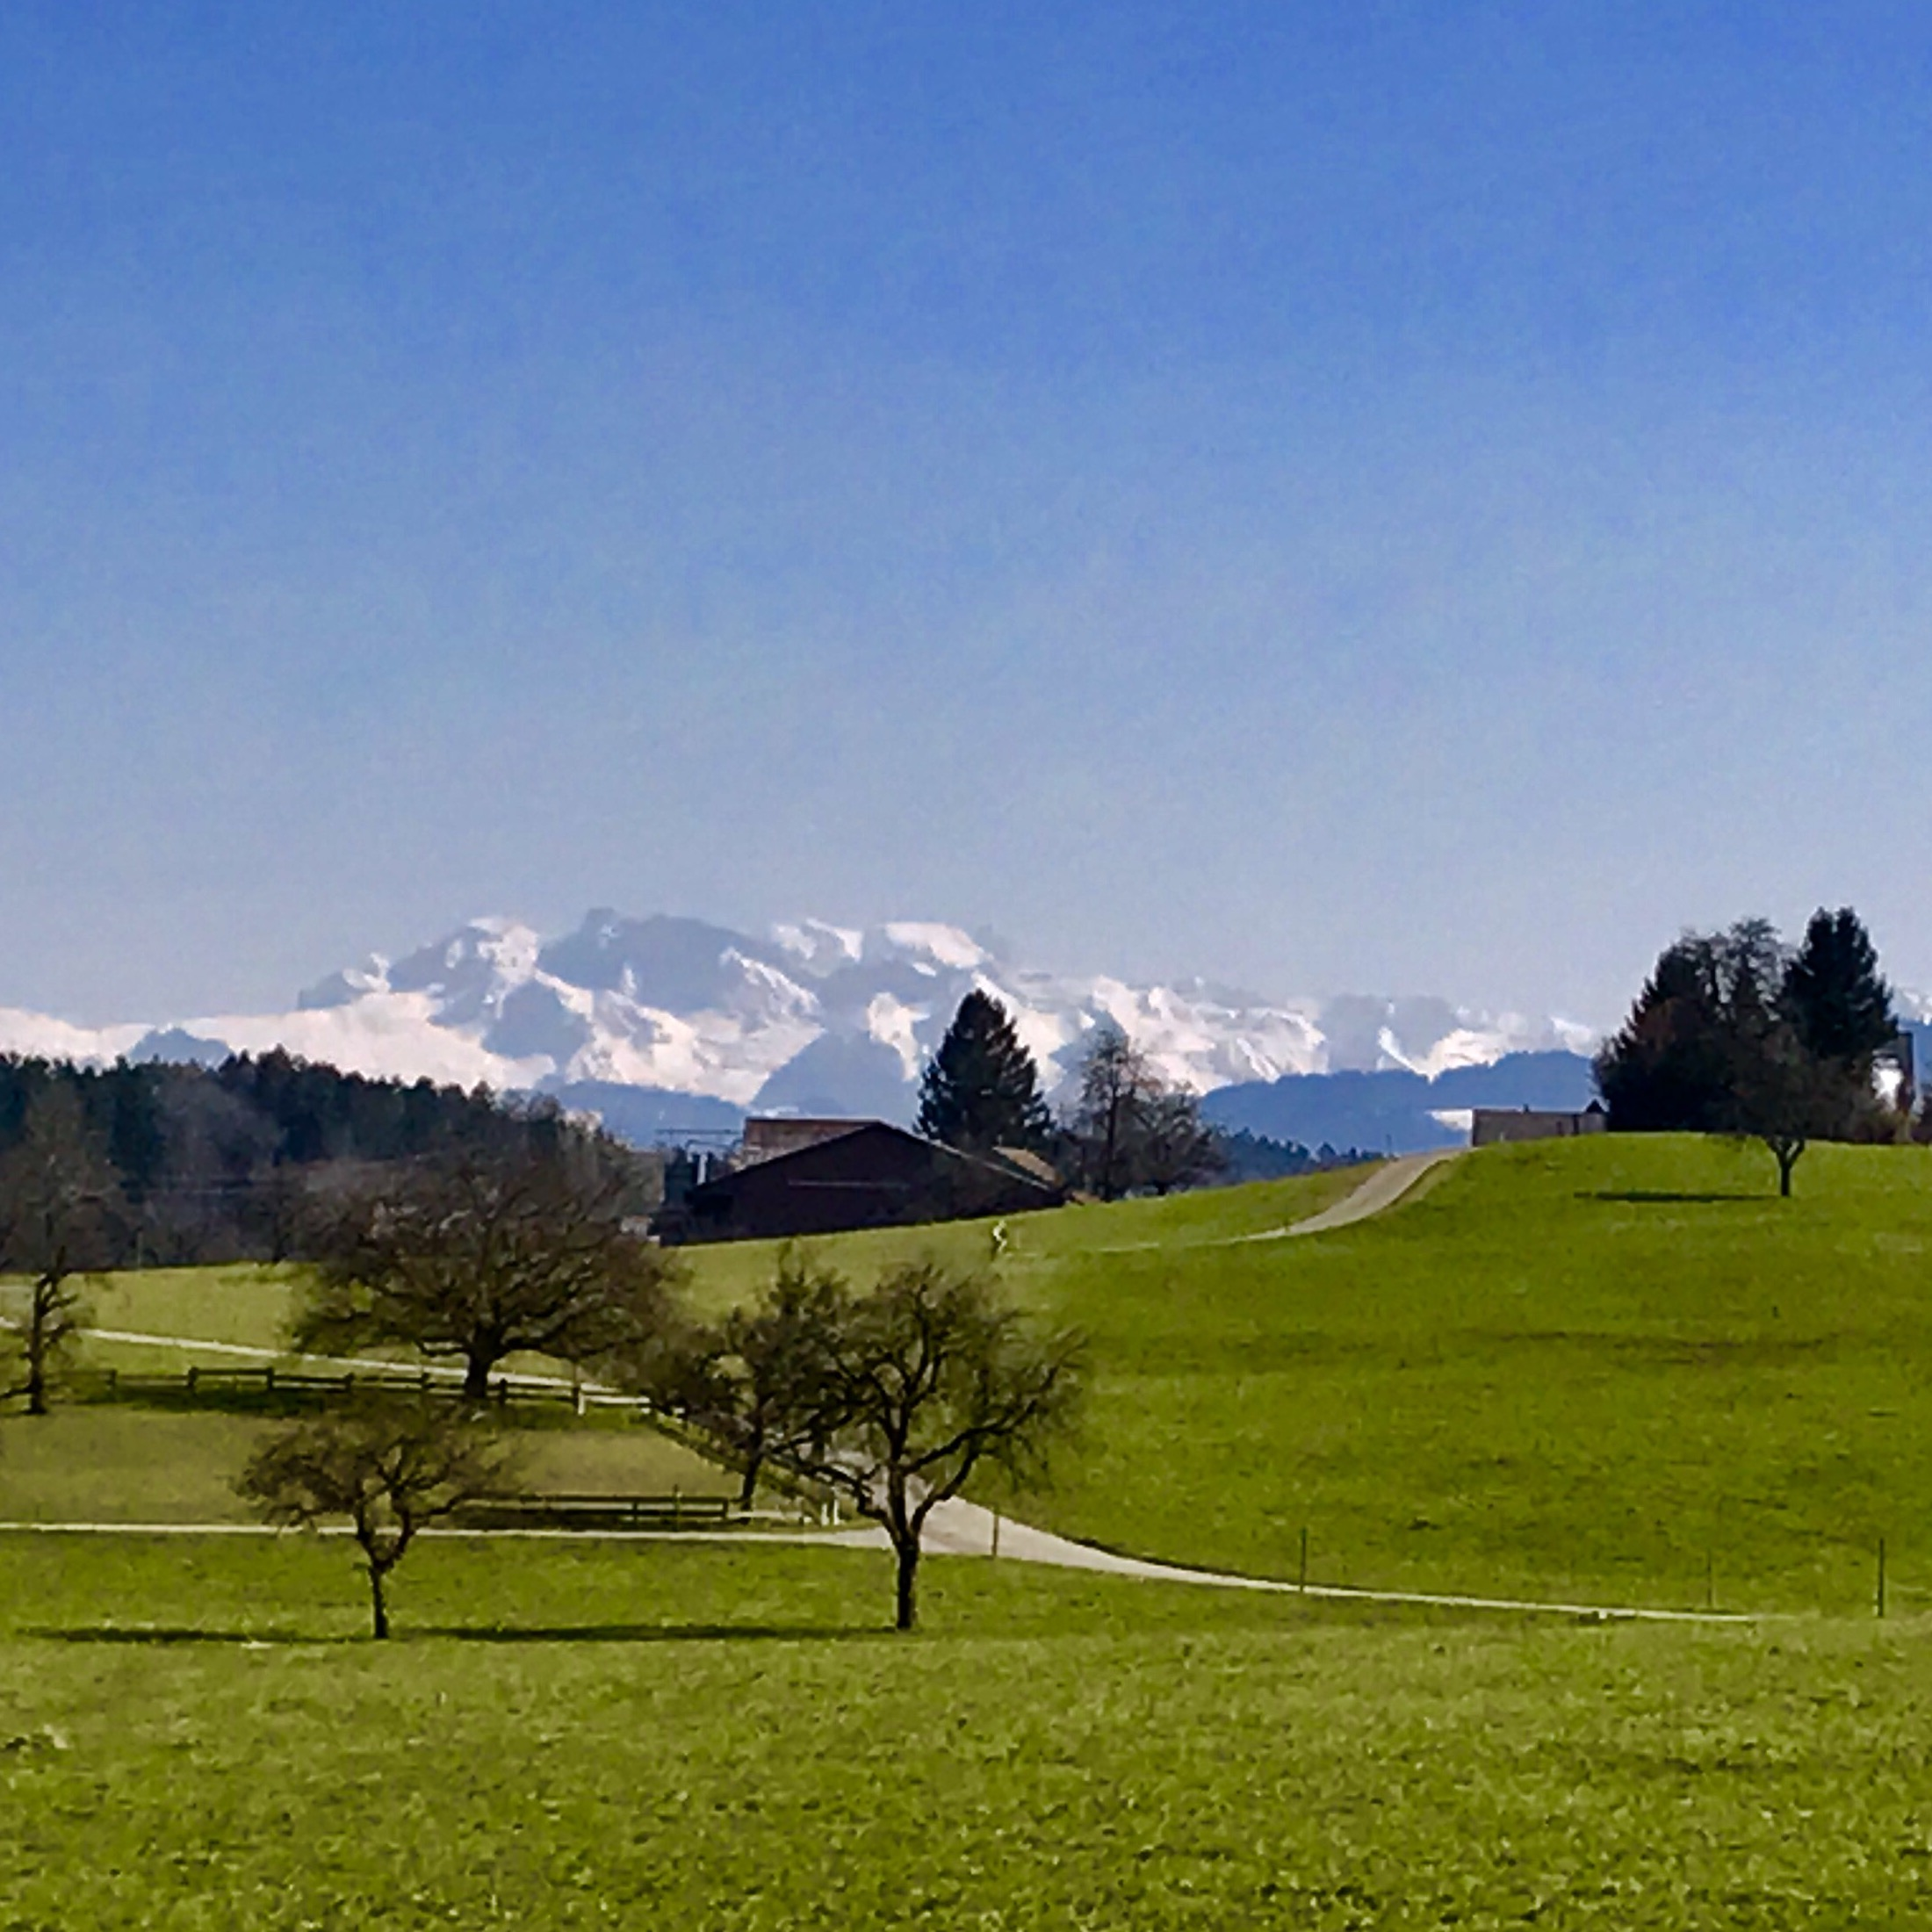
\includegraphics[width=\figfig\textwidth]{1-01-0.jpg}
	}
	\subbottom[image after segmentation\label{fig:egaftseg}]{
		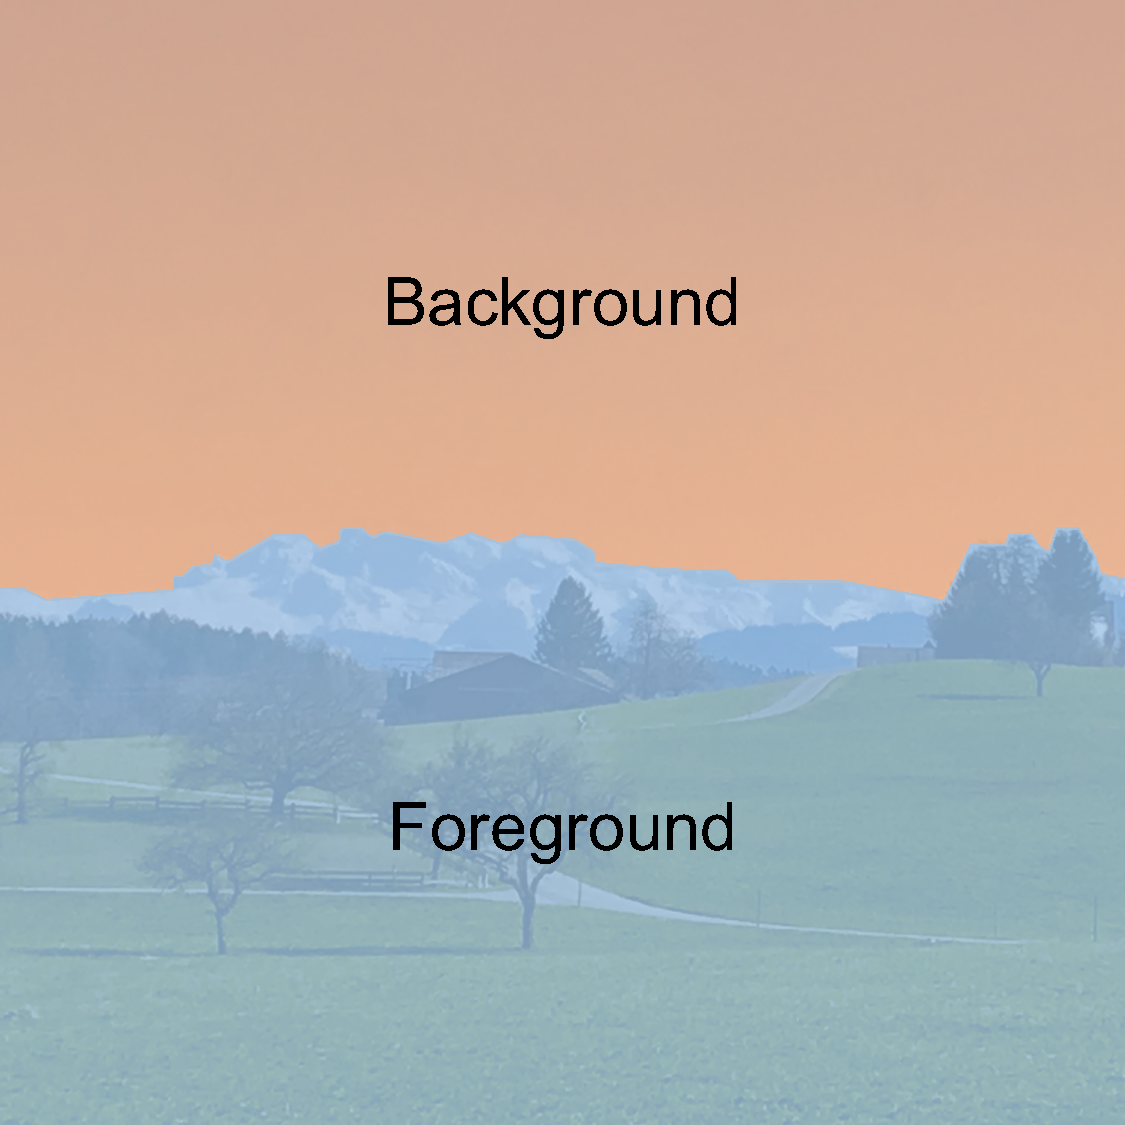
\includegraphics[width=\figfig\textwidth]{1-01-1.pdf}
	}
    \caption[Example of binary image segmentation]{Example of image binary segmentation. The original image (a) is taken from Uetzgi Takeoff.}
	\label{fig:eg01imgseg}
\end{figure}

\subsection{Geometrical Shape}\label{geosha}

However, the pixel-wise representation introduced in subsection \ref{imgseg} has many limitations, such as the inability to locate the building, and requirement for relatively more storage. We want to get rid of the pixel-wise labelling and describe geometrical shape of each super-pixel in an image directly. The geometrical shape here generally refers to a polygon represented by a series of vectors or coordinates.

Deviating from the standard paradigm of labeling pixels and aiming to directly learn the geometry of the buildings have following advantages: (1) polygon representation has much less redundancy than pixel-wise labelling; (2) polygon representation has relatively less storage than pixel-wise labelling; (3) polygon representation can be expressed in vectors and used at different levels so that buildings and other objects can be modeled more naturally; (4) the polygons learned can be directly marked in the electronic map, but the pixels can not.

The polygon representation is therefore a more compact and useful representation. Recently, deep learning methods have demonstrated remarkable achievements in image segmentation tasks. The related methods have already been applied to aerial images [10,11,12,13,14]. However, these traditional CNN architectures are still limited to conventional grid structure diagrams and their output is still pixel-wise. So, how to quickly detect geometrical shapes from aerial images has become a big problem.

In short, the purpose of this project is to develop novel deep learning methods for the geometry of graphs and arbitrary structures, and we want to introduce object topologies and shapes into deep learning techniques.

\section{Problem Definition}\label{prodef}

\paragraph{Goal of Project} Given an aerial image, our goal is to extract the polygon shape for each building in the satellite image. Input is an satellite image, denoting 
\begin{equation}
I = \{I_{ijk}\}_{i \in \{1,2,\ldots,h\}, j \in \{1,2,\ldots,w\}, k \in \{1,2,3\}},
\end{equation}
where $I_{ijk}$ denotes the pixel value of $i$-th row, $j$-th column and $k$-th channel in the image, $w$ and $h$ denote image's width and height, and output is polygons, denoting
\begin{equation}
P = \{P^{(n)}\}_{n \in \{1,2,\ldots,N\}},
\end{equation}
\begin{equation}
P^{(n)} = \{(i^{(n)}_t, j^{(n)}_t)\}_{t \in \{1,2,\ldots,l_n\}},
\end{equation}
where $N$ denotes the number of buildings in the image, $P^{(n)}$ and $l_n$ denote the $n$-th polygon and its number of vertices, $i^{(n)}_t$ and $j^{(n)}_t$ denote the image coordinates of $t$-th vertex of the polygon $P^{(n)}$ in the original image.

\section{Focus of This Work}\label{fcswrk}

The problem is challenging because it requires the correct detection of all buildings in an aerial image while also precisely segmenting each instance in the form of polygon. It therefore combines elements from the classical computer vision tasks of object detection, where the goal is to classify individual objects and localize each using a bounding box, and geometrical segmentation, where the goal is to extract polygon.

In order to solve this problem, we propose a new model, \modelnameshort\ (\modelnamelong), which is a combination of the FPN (Feature Pyramid Network) part in Mask R-CNN and PolygonRNN. FPN is used to localize buildings, i.e. to detect the RoIs (Regions of Interest) in the image, and PolygonRNN is used to find geometrical shapes.

\section{Thesis Organization}\label{thsorg}

This thesis is organized as follows. Chapter 2 reviews related work, focuses on the pixel-wise segmentation method and rotated bounding boxes regression method used in previous theses, and also introduces two recent new models, Mask R-CNN and PolygonRNN. In chapter 3, the specific architectures of the two new models are be discussed, and the structure of our proposed model is also explained in detail. Chapter 4 describes the dataset we use and gives the experiment results. Finally, chapter 5 makes conclusions, points out the problems exist in our project and gives future direction.

Following common terminology, we use object detection to denote detection via bounding boxes, not masks, and semantic segmentation to denote pixel-wise classification without differentiating instances. Yet we note that instance segmentation is both semantic and a form of detection.
